\section{Basic Principles}
\subsection{Nodes and Layers}
The fundamental building block of neural networks are nodes, which often is analogously seen as an neuron from in a brain, hence the name neural network. In a node we have the bias and the activation function and a weight for each connected node.

\begin{figure}[H]
    \centering
    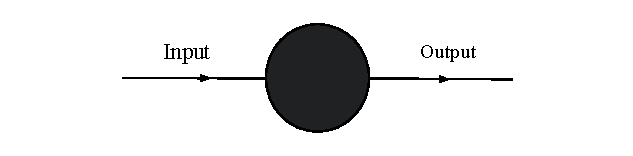
\includegraphics{Figures/Drawn/machinelearning/onenode.pdf}
    \caption{A singular node. Has an input which is affected by the weight, bias and activation function within the node.}
    \label{fig:onenode}
\end{figure}

In the figure above the node takes in a input from the left, $x$. The weight, $w$, and bias, $b$, create the intermediate output of the node accordingly:

\begin{equation}
    n = wx + b \; .
\end{equation}

Then $n$ is passed through an activation function, $\sigma$ and we get the output of the node

\begin{equation}
    z = \sigma \left ( n \right ) \; .
\end{equation}

Combining several nodes which takes the same input we get a layer. Layers are then connected where the previous layer's output is sent as input to the next via these connections. This is the simplest network, called a feedforward network, as we pass the input through layer by layer without any inter-layer connections.

\begin{figure}[H]
    \centering
    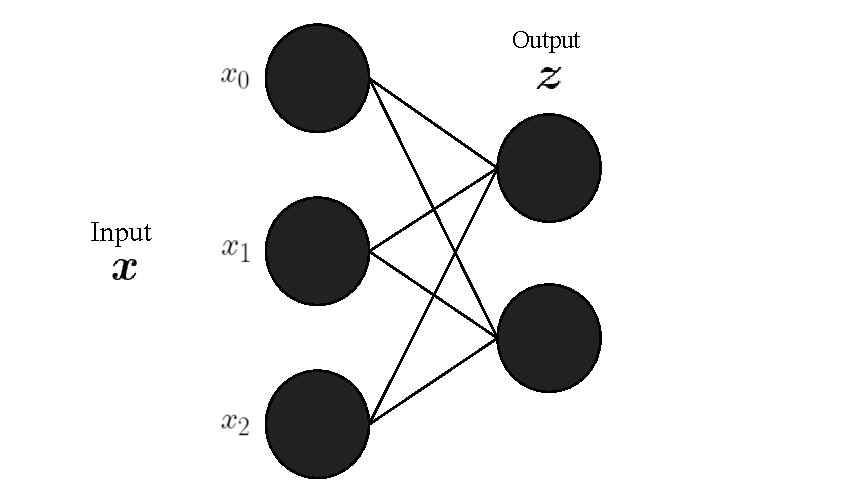
\includegraphics[width=\textwidth]{Figures/Drawn/machinelearning/inputoutputlayer.pdf}
    \caption{A simple feedforward neural network where we have an input layer, individual connections to the input, and a output layer. The output layer's nodes are all connected to each of the input layer's nodes.}
    \label{fig:inputoutput}
\end{figure}

Here the first layer is called an input layer as it has a one to one correspondence with a input data point. The input and output layer is fully connected however, where the output of each of the input layer's nodes are sent to each of the output layer's, where each connection has its own weight. Using vectors to represent the layers we have

\begin{equation}
    \boldsymbol{x} = \begin{bmatrix}
        x_0 \\ x_1 \\ x_2
    \end{bmatrix}
\end{equation}

as input, which is then inserted in the input layer's nodes as shown in \ref{fig:inputoutput}. The weights now has an extra dimension as each nodes is connected to each node in the next layer, so we can represent it with a matrix:

\begin{equation}
    W = \begin{bmatrix}
        w_{00} &  w_{10} & w_{20} \\
       w_{01} & w_{11} & w_{21}
      
    \end{bmatrix} \;
\end{equation}

where the weight $w_{kj}$ is the weight of the connection between node $k$ of the input layer and node $j$ of the output layer. Feeding the input forward we first get the intermediate output

\begin{equation}\label{eq:feedforward}
    \boldsymbol{n} = W \boldsymbol{x} + \boldsymbol{b} 
\end{equation}

where we use simple matrix multiplication. The output layer often has a unique activation function to make the output more applicable to a certain context. For example, in classification problems the softmax function

\begin{equation}
    \sigma_{s} (\boldsymbol{z}' )_{i}={\frac {e^{z'_{i}}}{\sum _{j=1}^{N}e^{z'_{j}}}} \; ,
\end{equation}

which normalizes the output to a probability distribution, is often used. Using the softmax activation function, we have the final output

\begin{equation}
    \boldsymbol{z} = \sigma_s \left ( \boldsymbol{n} \right ) \; .
\end{equation}

The network model is easily expandable to more layers as one just sends the output of a layer into the next by following equation \ref{eq:feedforward}.

\subsection{Activation function}

 The term activation function is inspired from the way biological neurons 'activate' after a certain signal threshold is met. The activation function chosen for a given network can have large impact on the finished trained model. Some common activation functions are 

\setlength{\tabcolsep}{25pt}
\begin{table}[H]
\begin{center}
\begin{tabular}{l c}
 \makecell{ReLU \\ $max \left ( 0, x \right )$} & \raisebox{-.5\height}{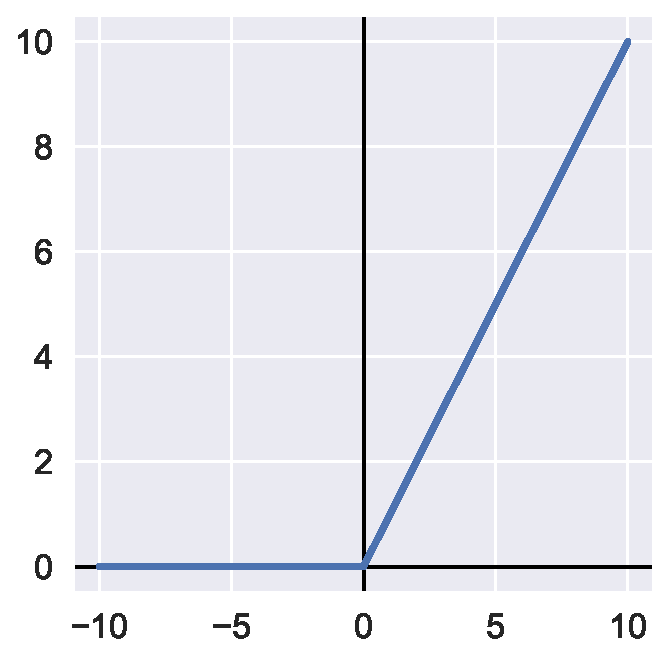
\includegraphics[width=0.5\textwidth]{Figures/Plots/machinelearning/curve1.pdf}}
\end{tabular}
\end{center}
\vspace{-4mm}
\end{table}

The Rectified Linear Unit activation function is one of the most basic activation functions. Since it does not have an upper bound, the activation function can have problems with values becoming too large. ReLU is however one of the most popular activation function because it has an derivative easy to calculate and avoids the vanishing gradient problem during learning.

\setlength{\tabcolsep}{6pt}
\begin{table}[H]
\begin{center}
\begin{tabular}{l c}
 \makecell{Leaky ReLU  \\ $max \left ( ax, x \right ) \; a \in \left < 0, 1 \right > $} & \raisebox{-.5\height}{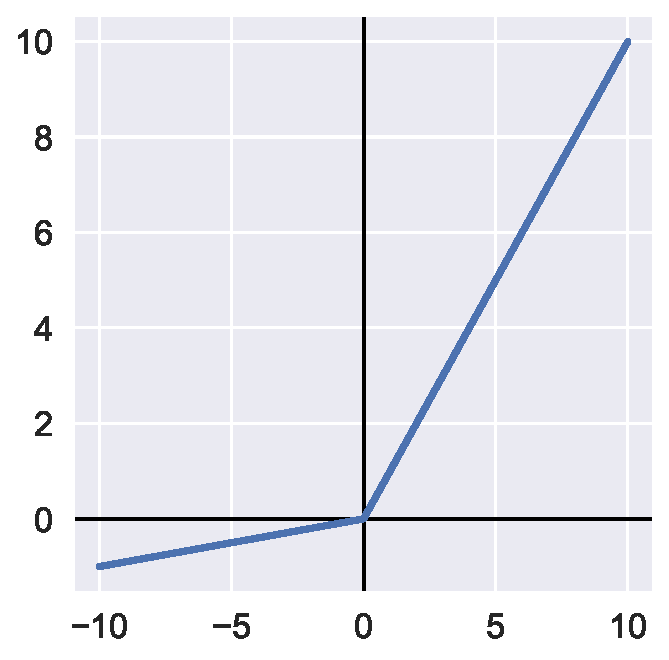
\includegraphics[width=0.5\textwidth]{Figures/Plots/machinelearning/curve2.pdf}}
\end{tabular}
\end{center}
\vspace{-4mm}
\end{table}

Leaky ReLU adds the possibility for negative values to impact the output of the node.

\setlength{\tabcolsep}{23pt}
\begin{table}[H]
\begin{center} 
\begin{tabular}{l c}
 \makecell{Sigmoid  \\ $\sigma \left ( x \right ) = \frac{1}{1+e^{-x}}$} & \raisebox{-.5\height}{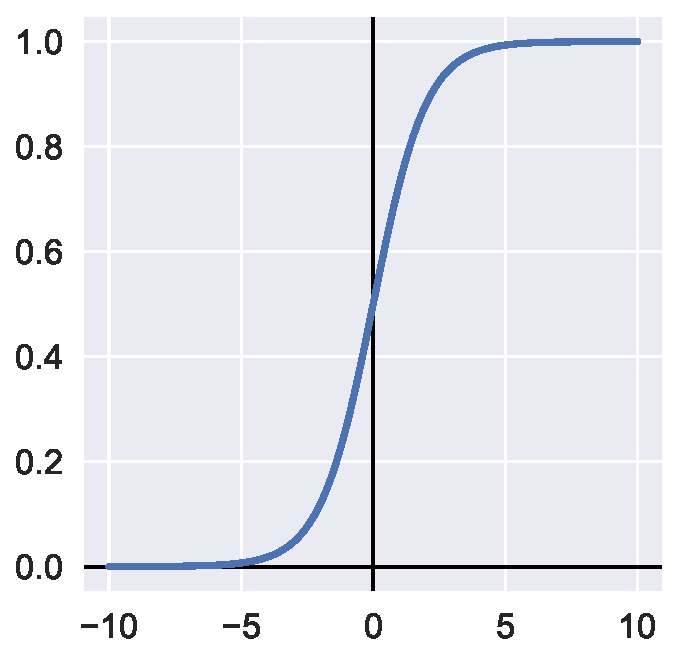
\includegraphics[width=0.5\textwidth]{Figures/Plots/machinelearning/curve0.pdf}}
\end{tabular}
\captionof{table}{\label{Tab:sigmoid}}
\end{center}
\vspace{-4mm}
\end{table}
\setlength{\tabcolsep}{6pt}

The Sigmoid activation function has both a upper and lower bound, preventing the values from escalating out of control, but has an more computationally expensive derivative and can struggle with the vanishing gradient problem during learning.

\subsection{Training a neural network}

Training a neural network is done by changing the weights and biases such that the output comes closer to a desired goal. This goal is to minimize a cost function $C$, which can be any function. As an example, an common cost function for regression is the squared error

\begin{equation}
    C = \sum_k \left ( t_k - z_k \right )^2
\end{equation}

where $t$ is a target value and $z$ is the model output. We want to change the weights and biases in such a way that the cost function decreases. A natural way would be to use the gradient of the cost function in terms of the weights and biases, and decrease the variables by a proportional amount, such that we approach the minima of the cost function. Finding the gradient of the cost function in terms of the weights and biases is done by backpropagation, a method introduced by S. Linnainmaa in 1960 \cite{RosenblattBack}, completed by F. Rosenblatt in 1976 \cite{Linnainmaa1976} and popularized by D. E. Rumelhart in 1982 \cite{Rumelhart1986}. The method is derived by application of the chain rule starting from the output and going layer by layer to get to the input. 

We expand our simple input-output model \ref{fig:inputoutput} and define a subscript for the different layers and nodes as shown here:

\begin{figure}[H]
    \centering
    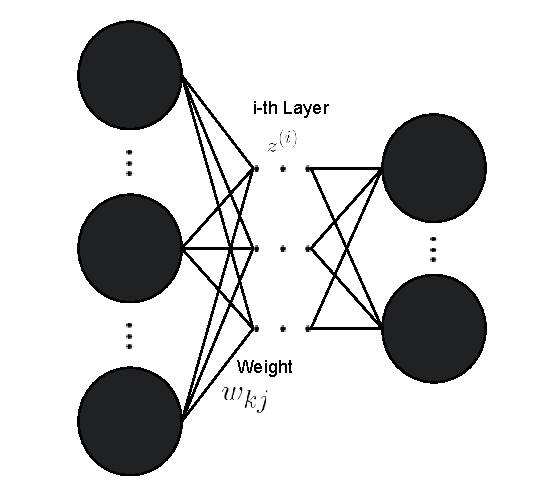
\includegraphics{Figures/Drawn/machinelearning/generalnetwork.pdf}
    \caption{A more general network where we $w_{kj}$ is the weight matrix}
    \label{fig:gennet}
\end{figure}

We have that:

\begin{description}
    \item[$\boldsymbol{z}^{(i)}$] is the i-th layer vector output. $(i)$ is the layer subscript, going from the input layer $z^{(0)}$ to the output layer $z^{(L)}$.
    \item[$\boldsymbol{n}$] is the intermediate output of a layer before it is sent through an activation function.
    \item[$\sigma$] is an activation function.
    \item[$W^{(i)}$] is a weight matrix with weights $w_{kj}$, which is the weight from $k$-th node of the $i$-th layer to node $j$ of layer $i+1$.
     
\end{description}

Starting from the output we want to find

\begin{equation}
    \Delta W^{(L-1)} = -\eta\frac{\partial C}{\partial W^{(L-1)}} \; ,
\end{equation}

where $\eta$ is a chosen learning rate. The change in a single weight

\begin{equation}
    \Delta w_{kj}^{(L-1)}  = -\eta \frac{\partial C}{\partial w_{kj}^{(L-1)}} \; ,
\end{equation}

where we can add the dependency on the activation function and intermediate output

\begin{equation}
    \Delta w_{kj}^{(L-1)} = -\eta \frac{\partial C}{\partial z_k^{(L)}}\frac{\partial z_k^{(L)}}{\partial n_k^{(L)}}\frac{\partial n_k^{(L)}}{\partial w_{kj}^{(L-1)}}
\end{equation}

Where we have that

\begin{equation}
    \frac{\partial C}{\partial z_k^{(L)}} = - 2 \left ( t_k - z_k^{(L)} \right )
\end{equation}

and using the sigmoid activation function, \ref{Tab:sigmoid}, we have

\begin{equation} \label{eq:outnet}
    \frac{\partial z_k^{(L)}}{\partial n_k^{(L)}} = \frac{\partial \left ( \frac{1}{1 = e^{-n_k}} \right )}{\partial n_k} = \frac{e^{-n_k}}{\left (1+e^{-n_k} \right ) ^2} = n_k(1-n_k)
\end{equation}

 and then lastly the intermediate output 
 
\begin{equation} \label{eq:netweight}
    \frac{\partial n_k^{(L)}}{\partial w_{kj}^{(L-1)}} = \frac{\partial \left ( w_{kj}^{(L-1)} z_j^{(L-1)} + b_j^{(L-1)} \right )}{\partial  w_{kj}^{(L-1)}} = z_j^{(L-1)}
\end{equation}

So we can write the change of weight as

\begin{equation}
    \Delta w_{kj}^{(L-1)} = \eta \left ( t_k - z_k^{(L)} \right ) z_k^{(L)} \left ( 1 - z_k^{(L)} \right ) z_j^{(L-1)}  \; .
\end{equation}

We simplify by defining

\begin{equation}
    \delta_k^{(L)} = \left ( t_k - z_k^{(L)} \right ) z_k^{(L)} \left ( 1 - z_k^{(L)} \right ) \;
\end{equation}

and get

\begin{equation}
    \Delta w_{kj}^{(L-1)} = \eta \delta_k^{(L)} z_j^{(L-1)}  \; ,
\end{equation}

where we have shortened the $-2$ factor into $\eta$ as well. For the next layer, $(L-2)$, we have that a individual node is connected to each of the previous layer's nodes. We then have the change

\begin{equation}
    \Delta w_{jm}^{(L-2)} = \eta \left [ \sum_k \frac{\partial C}{\partial z_k^{(L)}}\frac{\partial z_k^{(L)}}{\partial n_k^{(L)}} \frac{\partial n_k^{(L)}}{\partial z_j^{(L-1)}}\right ] \frac{\partial z_j^{(L-1)}}{\partial n_j^{(L-1)}} \frac{\partial n_j^{(L-1)}}{\partial w_{jm}^{(L-2)}} \; ,
\end{equation}

where we have calculated the expression within the sum already

\begin{equation}
    \frac{\partial C}{\partial z_k^{(L)}}\frac{\partial z_k^{(L)}}{\partial n_k^{(L)}} \frac{\partial n_k^{(L)}}{\partial z_j^{(L-1)}} = \left ( t_k - z_k^{(L)} \right )z_k^{(L)}\left (1-z_k^{(L)} \right ) w_{kj}^{(L-1)} = \delta_k^{(L)} w_{kj}^{(L-1)} \; . 
\end{equation}

The expression outside the sum is calculated as in \ref{eq:outnet} and \ref{eq:netweight}

\begin{equation}
     \frac{\partial z_j^{(L-1)}}{\partial n_j^{(L-1)}} \frac{\partial n_j^{(L-1)}}{\partial w_{jm}^{(L-2)}} = z_j^{(L-1)} \left ( 1 - z_j^{(L-1)} \right  ) z_m^{(L-2)} \; .
\end{equation}

We can then write the change in weight as

\begin{equation}
   \Delta w_{jm}^{(L-2)} = \eta \left [ \sum_k \delta_k^{(L)} w_{kj}^{(L-1)} \right ] z_j^{(L-1)} \left ( 1 - z_j^{(L-1)} \right  ) z_m^{(L-2)} \; ,
\end{equation}

which we can further simplify by defining

\begin{equation}
    \delta_j^{(L-1)} = \left [ \sum_k \delta_k^{(L)} w_{kj}^{(L-1)} \right ] z_j^{(L-1)} \left ( 1 - z_j^{(L-1)} \right  )
\end{equation}

and we get

\begin{equation}
    \Delta w_{jm}^{(L-2)} = \eta \delta_j^{(L-1)} z_m^{(L-2)} \; .
\end{equation}

This process can then be repeated easily with the fact that

\begin{equation}
    \delta_k^{i-1} =  \left [ \sum_k \delta_k^{(i)} w_{kj}^{(i-1)} \right ] z_j^{(i-1)} \left ( 1 - z_j^{(i-1)} \right  ) 
\end{equation}

for any layers further in. 